% Primary source: https://arxiv.org/abs/1707.01926
\documentclass[tikz,border=5pt]{standalone}
\usepackage[T1]{fontenc}
\usepackage{lmodern,amsmath,amssymb}
\usetikzlibrary{arrows.meta,calc,positioning,fit,backgrounds,shapes.geometric,matrix,decorations.pathreplacing,patterns}
\definecolor{ink}{gray}{0.08}
\definecolor{wash}{gray}{0.965}
\definecolor{soft}{gray}{0.45}
\tikzset{box/.style={draw=ink,line width=.65pt,fill=white,align=center,inner sep=4pt,outer sep=0pt,font=\small},flow/.style={draw=ink,line width=.65pt,-{Latex[length=1.8mm,width=1.3mm]},rounded corners=2pt},annotation/.style={font=\scriptsize,text=soft,align=center},groupbox/.style={draw=soft,dashed,line width=.45pt,fill=wash}}
\begin{document}
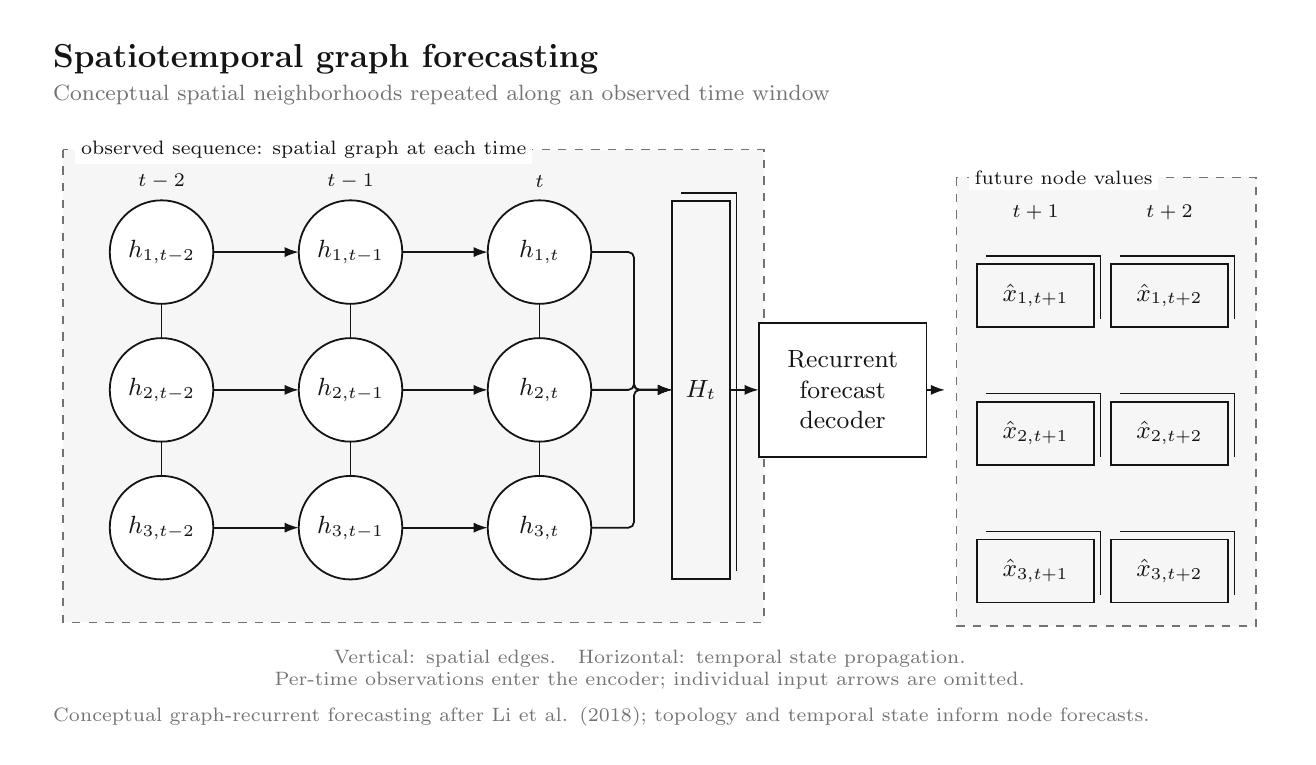
\begin{tikzpicture}[x=1cm,y=-1cm,font=\rmfamily,text=ink]

\path[use as bounding box] (0,0) rectangle (16,9);
\node[anchor=west,font=\large\bfseries] at (.2,.4) {Spatiotemporal graph forecasting};
\node[anchor=west,font=\footnotesize,text=soft] at (.2,.85) {Conceptual spatial neighborhoods repeated along an observed time window};
\begin{pgfonlayer}{background}
\draw[groupbox] (0.45,1.55) rectangle (9.35,7.55);
\node[anchor=west,font=\scriptsize,fill=white,inner sep=2pt] at (0.6,1.55) {observed sequence: spatial graph at each time};
\draw[groupbox] (11.8,1.9) rectangle (15.600000000000001,7.6);
\node[anchor=west,font=\scriptsize,fill=white,inner sep=2pt] at (11.950000000000001,1.9) {future node values};
\end{pgfonlayer}
\node[box,circle,minimum width=1.15cm,minimum height=1.15cm,text width=0.8999999999999999cm] (h11) at (1.7,2.85) {$h_{1,t-2}$};
\node[box,circle,minimum width=1.15cm,minimum height=1.15cm,text width=0.8999999999999999cm] (h21) at (1.7,4.6) {$h_{2,t-2}$};
\node[box,circle,minimum width=1.15cm,minimum height=1.15cm,text width=0.8999999999999999cm] (h31) at (1.7,6.35) {$h_{3,t-2}$};
\node[box,circle,minimum width=1.15cm,minimum height=1.15cm,text width=0.8999999999999999cm] (h12) at (4.1,2.85) {$h_{1,t-1}$};
\node[box,circle,minimum width=1.15cm,minimum height=1.15cm,text width=0.8999999999999999cm] (h22) at (4.1,4.6) {$h_{2,t-1}$};
\node[box,circle,minimum width=1.15cm,minimum height=1.15cm,text width=0.8999999999999999cm] (h32) at (4.1,6.35) {$h_{3,t-1}$};
\node[box,circle,minimum width=1.15cm,minimum height=1.15cm,text width=0.8999999999999999cm] (h13) at (6.5,2.85) {$h_{1,t}$};
\node[box,circle,minimum width=1.15cm,minimum height=1.15cm,text width=0.8999999999999999cm] (h23) at (6.5,4.6) {$h_{2,t}$};
\node[box,circle,minimum width=1.15cm,minimum height=1.15cm,text width=0.8999999999999999cm] (h33) at (6.5,6.35) {$h_{3,t}$};
\node[box,fill=wash,minimum width=0.7cm,minimum height=4.8cm,text width=0.44999999999999996cm] (state) at (8.55,4.6) {$H_t$};
\draw[ink,line width=.4pt] (8.3,2.0999999999999996) -- (9.0,2.0999999999999996) -- (9.0,6.9);
\node[box,minimum width=2.1cm,minimum height=1.7cm,text width=1.85cm] (decoder) at (10.35,4.6) {Recurrent\\forecast\\decoder};
\node[box,fill=wash,minimum width=1.45cm,minimum height=0.8cm,text width=1.2cm] (pred11) at (12.8,3.4000000000000004) {$\hat{x}_{1,t+1}$};
\draw[ink,line width=.4pt] (12.175,2.9000000000000004) -- (13.625,2.9000000000000004) -- (13.625,3.7);
\node[box,fill=wash,minimum width=1.45cm,minimum height=0.8cm,text width=1.2cm] (pred21) at (12.8,5.1499999999999995) {$\hat{x}_{2,t+1}$};
\draw[ink,line width=.4pt] (12.175,4.6499999999999995) -- (13.625,4.6499999999999995) -- (13.625,5.45);
\node[box,fill=wash,minimum width=1.45cm,minimum height=0.8cm,text width=1.2cm] (pred31) at (12.8,6.8999999999999995) {$\hat{x}_{3,t+1}$};
\draw[ink,line width=.4pt] (12.175,6.3999999999999995) -- (13.625,6.3999999999999995) -- (13.625,7.2);
\node[box,fill=wash,minimum width=1.45cm,minimum height=0.8cm,text width=1.2cm] (pred12) at (14.5,3.4000000000000004) {$\hat{x}_{1,t+2}$};
\draw[ink,line width=.4pt] (13.875,2.9000000000000004) -- (15.325,2.9000000000000004) -- (15.325,3.7);
\node[box,fill=wash,minimum width=1.45cm,minimum height=0.8cm,text width=1.2cm] (pred22) at (14.5,5.1499999999999995) {$\hat{x}_{2,t+2}$};
\draw[ink,line width=.4pt] (13.875,4.6499999999999995) -- (15.325,4.6499999999999995) -- (15.325,5.45);
\node[box,fill=wash,minimum width=1.45cm,minimum height=0.8cm,text width=1.2cm] (pred32) at (14.5,6.8999999999999995) {$\hat{x}_{3,t+2}$};
\draw[ink,line width=.4pt] (13.875,6.3999999999999995) -- (15.325,6.3999999999999995) -- (15.325,7.2);
\begin{pgfonlayer}{background}
\draw[flow,-] (h11.south) -- (h21.north);
\draw[flow,-] (h21.south) -- (h31.north);
\draw[flow,-] (h12.south) -- (h22.north);
\draw[flow,-] (h22.south) -- (h32.north);
\draw[flow,-] (h13.south) -- (h23.north);
\draw[flow,-] (h23.south) -- (h33.north);
\draw[flow] (h11.east) -- (h12.west);
\draw[flow] (h12.east) -- (h13.west);
\draw[flow] (h21.east) -- (h22.west);
\draw[flow] (h22.east) -- (h23.west);
\draw[flow] (h31.east) -- (h32.west);
\draw[flow] (h32.east) -- (h33.west);
\draw[flow] (h13.east) -- (7.7,2.85) -- (7.7,4.6) -- (state.west);
\draw[flow] (h23.east) -- (7.7,4.6) -- (7.7,4.6) -- (state.west);
\draw[flow] (h33.east) -- (7.7,6.35) -- (7.7,4.6) -- (state.west);
\draw[flow] (state.east) -- (decoder.west);
\end{pgfonlayer}
\node[font=\scriptsize] at (1.7,1.95) {$t-2$};
\node[font=\scriptsize] at (4.1,1.95) {$t-1$};
\node[font=\scriptsize] at (6.5,1.95) {$t$};
\node[font=\scriptsize] at (12.8,2.35) {$t+1$};
\node[font=\scriptsize] at (14.5,2.35) {$t+2$};
\draw[flow] (decoder.east) -- (11.65,4.6);
\node[annotation,text width=14.3cm] at (7.9,8.15) {Vertical: spatial edges.\quad Horizontal: temporal state propagation.\\Per-time observations enter the encoder; individual input arrows are omitted.};
\node[anchor=west,align=left,font=\scriptsize,text=soft,text width=15.6cm] at (.2,8.75) {Conceptual graph-recurrent forecasting after Li et al. (2018); topology and temporal state inform node forecasts.};
\end{tikzpicture}
\end{document}
